\documentclass[letterpaper, 10 pt, conference]{ieeeconf}  % Comment this line out if you need a4paper
%\documentclass[a4paper, 10pt, conference]{ieeeconf}      % Use this line for a4 paper

\IEEEoverridecommandlockouts                              % This command is only needed if 
                                                          % you want to use the \thanks command
\overrideIEEEmargins                                      % Needed to meet printer requirements.

%In case you encounter the following error:
%Error 1010 The PDF file may be corrupt (unable to open PDF file) OR
%Error 1000 An error occurred while parsing a contents stream. Unable to analyze the PDF file.
%This is a known problem with pdfLaTeX conversion filter. The file cannot be opened with acrobat reader
%Please use one of the alternatives below to circumvent this error by uncommenting one or the other
%\pdfobjcompresslevel=0
%\pdfminorversion=4

% See the \addtolength command later in the file to balance the column lengths
% on the last page of the document

% The following packages can be found on http:\\www.ctan.org
\usepackage{graphicx} % for pdf, bitmapped graphics files
%\usepackage{epsfig} % for postscript graphics files
%\usepackage{mathptmx} % assumes new font selection scheme installed
%\usepackage{times} % assumes new font selection scheme installed
%\usepackage{amsmath} % assumes amsmath package installed
%\usepackage{amssymb}  % assumes amsmath package installed

\title{\LARGE \bf
Silver Spoon Effect on Education: Analysis of The Effect of Household Wealth Toward Children's Educational Output
}


\author{Hyecheol Jang$^{*1}$, Carleigh Heintz$^{*2}$, Chang Su$^{*3}$, Desmond Fung$^{*4}$, and Tsz Yau Iris Chow$^{*5}$% <-this % stops a space
\thanks{$^{*}$Everyone is an undergraduate student of the Department of  Statistics, University of Wisconsin - Madison (Madison, WI, 53706, USA), taking STAT 333 during FALL19, with professor Karl Rohe.}%
\thanks{$^{1}$Hyecheol Jang
        {\tt\small hyecheol.jang@wisc.edu}}%
\thanks{$^{2}$Carleigh Heintz
        {\tt\small cmheintz@wisc.edu}}%
\thanks{$^{3}$Chang Su
        {\tt\small csu29@wisc.edu}}%
\thanks{$^{4}$Desmond Fung
        {\tt\small dfung2@wisc.edu}}%
\thanks{$^{5}$Tsz Yau Iris Chow
        {\tt\small tchow7@wisc.edu}}%
}



\begin{document}

\maketitle
\thispagestyle{empty}
\pagestyle{empty}


%%%%%%%%%%%%%%%%%%%%%%%%%%%%%%%%%%%%%%%%%%%%%%%%%%%%%%%%%%%%%%%%%%%%%%%%%%%%%%%%
\begin{abstract}

This research shows the relationship between the wealthiness and willingness to invest toward the children's education and the educational output of those children.
We utilize mean income, private school enrollment rate, demographics, and employees' highest diploma for an area as features and ACT score and high school graduation rate of people between 18 and 24 years old as output to fit our linear regression model.

Showing the statistical significance of mean income, we verified that wealthiness affects academic success.
By combining the fact that people with higher degrees earns more money in future, the concerns about the silver spoon effect caused by education has been proved.

\end{abstract}


%%%%%%%%%%%%%%%%%%%%%%%%%%%%%%%%%%%%%%%%%%%%%%%%%%%%%%%%%%%%%%%%%%%%%%%%%%%%%%%%
\section{INTRODUCTION}

Nowadays, the majority of countries and societies are having a hard-time addressing long-resting social issues: polarization.
Modern society rarely has an identifying system, but due to the extreme polarization, it is not difficult to see separated “classes”, classified people’s life-style by wealthiness, in the real world.
With the instinct of mankind, everyone wants to be a part of upper-class society, and they, especially middle and lower class households believe education could be a ladder to go up to the upper class.
According to Rugarber (2017, [1]), the higher-education degree holder gained about 1.5 times higher salary compared to those who only have a high-school diploma.
Also, by showing two sets of data with different time-frames, in the years 1999 and 2015, Rugarber was able to address that the wage gap becomes wider over time (para. 1-3).
Seeing the previous analysis of the data, it looks like the higher educational status makes a higher salary, which lets people move toward the upper class.

However, education opportunities are not equally provided for all people in society.
With investment of additional resources on children’s education, paying tuition for private school, hiring tutors, and even sending their kids to other countries, people expect to bring better opportunity to their kids; therefore, education could be one of the ways to transfer the wealth of parents’ generation to their kids, making polarization even worse.
By conducting this research, we want to verify the existence of the "silver spoon effect" - if parents are wealthy, their kids are more likely to be wealthy - caused by education.
Specifically, we want to show that the areas with higher economic status and with the strong willingness of investing more on their next generations’ education have better educational output, expecting we can see a positive relationship between wealth and educational results (ACT Score, High School Graduation Rate, Statewide test score).
\textbf{Our analysis shows that areas with higher economic status have better educational output in Wisconsin}.

By showing the relatedness of wealth and educational output, we, ultimately, want to verify whether education might be used as a tool for “upper classes” to indirectly shift their capitals and superior societal position to the next generation.

\section{DATA COLLECTION / ANALYSIS}

Before going through how we collected and analyzed the datasets, note that all relevent dataset, codes, and documents are in our GitHub repository (URL: \textit{https://github.com/hyecheol123/STAT333-Edugression})

\subsection{Wisconsin Income by County}

Before analyzing the relationship between the economic status and the educational output, we started to make a graph of annual wage per employee for each county in Wisconsin.
This can be used gauge which citizens within the counties of the state are making more money compared to others, we are using this as a proxy variable for economic status.

The data has been retrieved from Bureau of Labor Statics (BLS)'s "Quarterly Census of Employment and Wages" data, and we used year 2017's census data (QCEW News Releases., n.d., [2]).

\textbf{Database search criteria} has been listed below.

\begin{itemize}

\item All Counties in a State, One Industry
\item Counties in Wisconsin
\item Year: 2017
\item Quarter: Annual Averages
\item Ownership: Total, All Ownerships
\item Industry: 10: Total, All Industries
\item Do not Include records with suppressed employment and wages

\end{itemize}
\vspace{1\baselineskip}

By selecting specific columns based on "QCEW Open Data Access: CSV Data Slices" (Data Slices by Industry., 2016, [3]), we are able to make two plots for "Total Annual Wage" and "Annual Wage per Employee" for each of the counties of the Wisconsin.
The unit of income has been measured in USD(U.S. Dollar) and the unit of analysis is counties (FIPS code).
Note that we understood the total/annual wage is synonym of total/annual income for each county, and from now on, this paper will use the term "income" as a synonym of wage, including the original meaning of the term income.

\begin{figure}[h]
\begin{center}
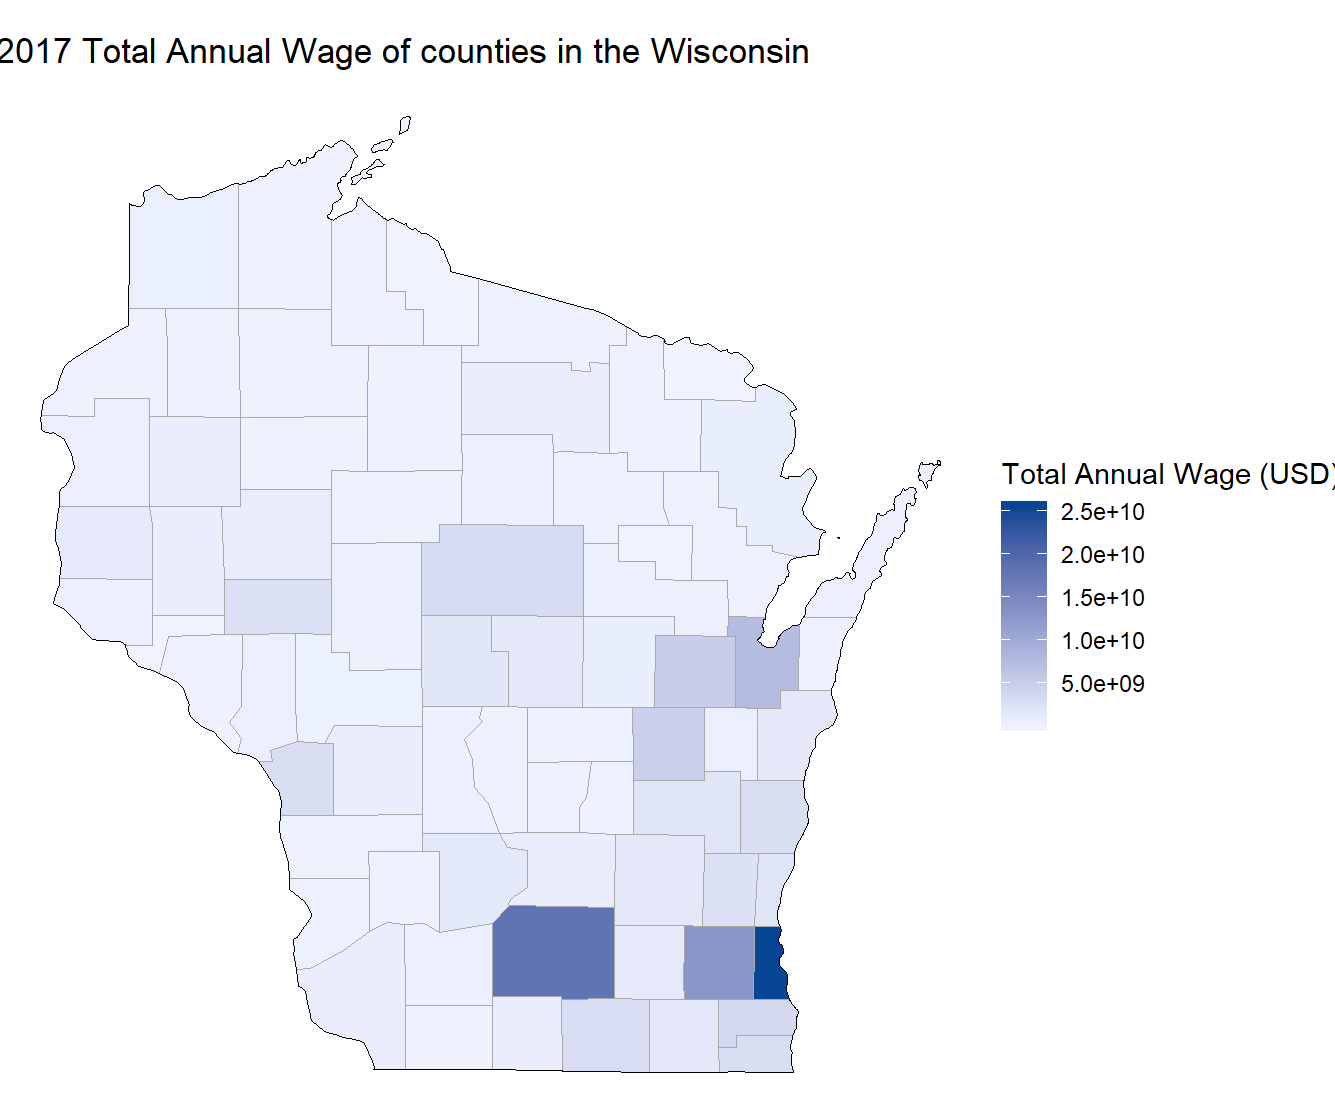
\includegraphics[width=1.0\linewidth]{2017_Total_Annual_Wage.png}
\end{center}
\caption{Plot for Total Annual Wage(Income) of counties in the Wisconsin}
\label{fig:long}
\label{fig:onecol}
\end{figure}

Seeing the plot for Total Annual Wage(Income) of counties in Wisconsin (Fig. 1), it can be concluded that the Madison and Milwaukee areas can be considered the economic centers of the Wisconsin, but as this plot indicated cumulative total wage that \textbf{all} workers in each county made, it does not consider the populations of each county, which allows for counties with larger populations to have much greater total wage than counties with smaller populations.

\begin{figure}[h]
\begin{center}
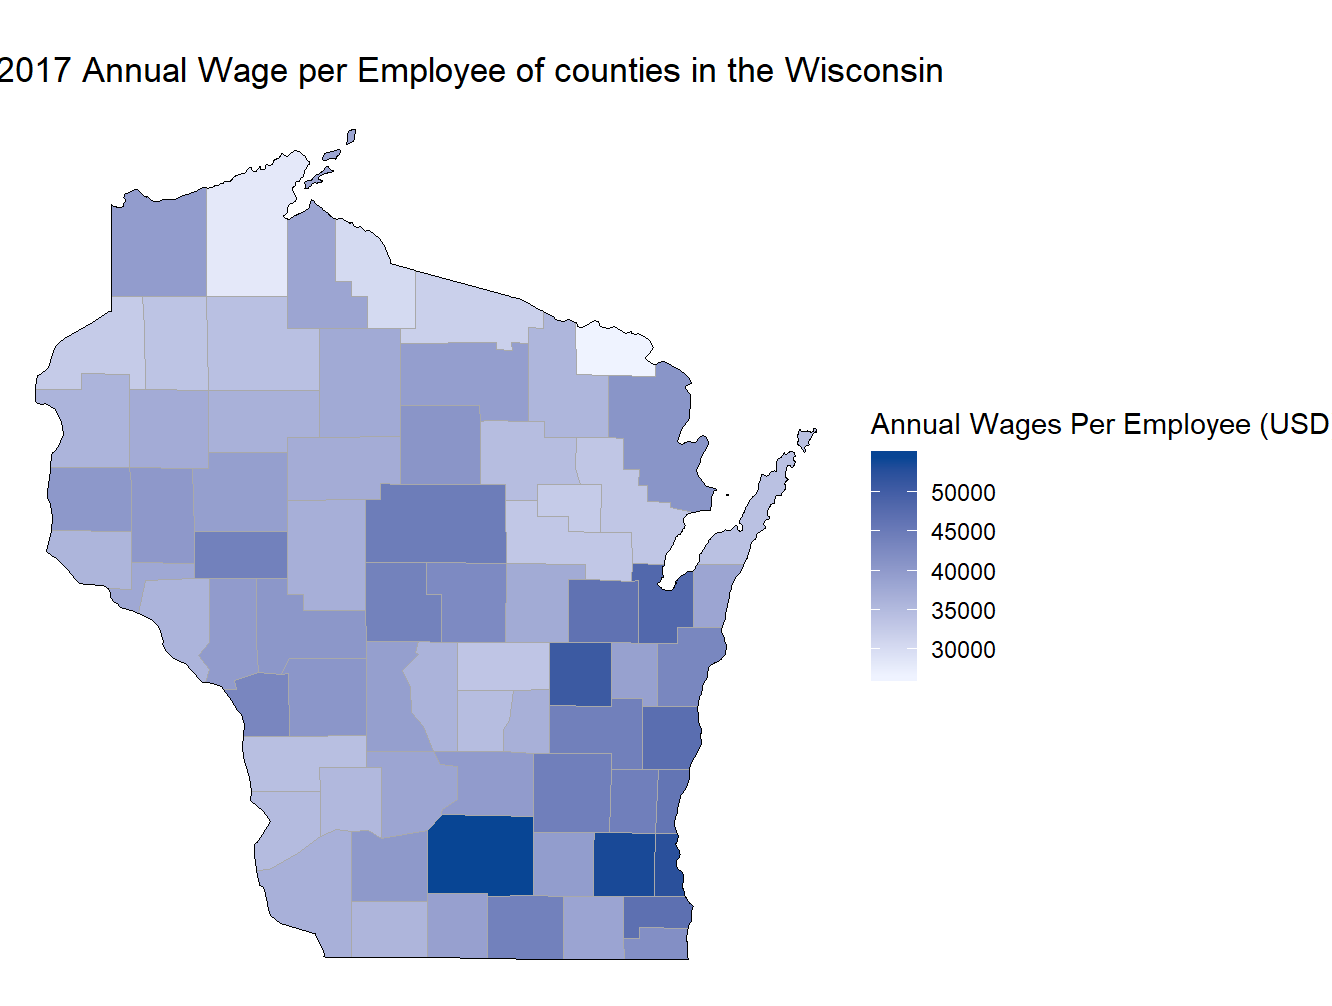
\includegraphics[width=1.0\linewidth]{2017_Annual_Wage_per_Employee.png}
\end{center}
\caption{Plot for Annual Wage(Income) per Employee of counties in the Wisconsin}
\label{fig:long}
\label{fig:onecol}
\end{figure}

Seeing the plot for Annual Wage(Income) per Employee of counties in Wisconsin (Fig. 2), it can still be concluded that the Madison and Milwaukee areas are considered as the economic center of the Wisconsin, but as this plot indicated average employee's income, it is more likely to represent household economic power compare to the previous plot.
Therefore, for further analysis, we decided to use average income to represent household economic status.

\subsection{Wisconsin Mean Income by zip code}

To get more specific data, our team decided to use data set coded by zip code.
To begin with, we analyzed the mean income for each zip code, which indicates household economic status.

The data has been retrieved from American Community Survey (ACS), and we specifically used year 2017's census data for Mean Income In The Past 12 Months (In 2017 Inflation-Adjusted Dollars) from 2013-2017 American Community Survey 5-Year Estimates (American FactFinder ..., 2010, [4]).
From the cited database, we used \textbf{search criteria} below.

\begin{itemize}

\item Table Name: S1902
\item Select 2017 data
\item Added Geographic after Search: 5-Digit Zip Code Tabulation Area - 860
\item State: Wisconsin
\item All 5-Digit Zip Code Tabulation Areas

\end{itemize}
\vspace{1\baselineskip}

By selecting Mean Income - Estimate for each zip code, we were able to get the mean income for each zip code.
The unit of income is USD, and the unit of analysis is each area using same zip code.

\begin{figure}[h]
\begin{center}
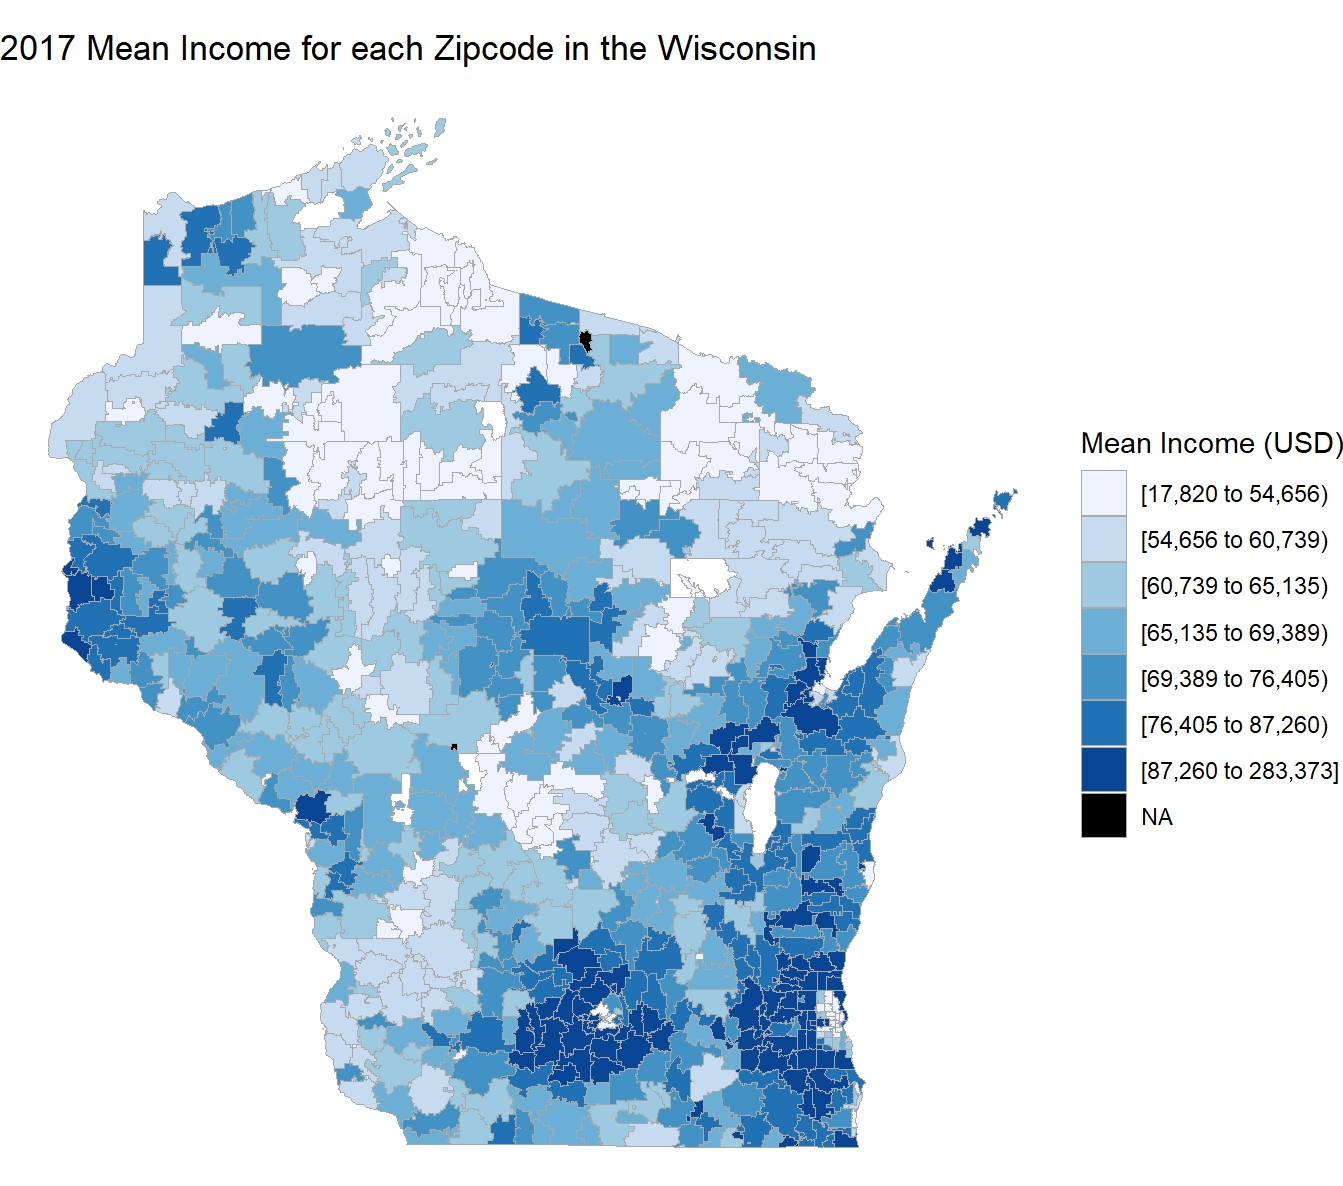
\includegraphics[width=1.0\linewidth]{2017_Mean_Income_Zipcode.jpg}
\end{center}
\caption{Plot for 2017 Mean Income for each Zip Code in the Wisconsin}
\label{fig:long}
\label{fig:onecol}
\end{figure}

Seeing the plot of wage coded by zip code (Fig. 3), we can still conclude that Madison and Milwaukee area's mean incomes are still higher than other areas.
However, we are able to intuitively see that there exist outliers in this data (See the legend), which is not represented in the plot clearly.

Looking through the data set, the area zip code 53047 is an outlier, where its mean income is reaching near 300 thousand, while others are less than 200 thousands.
After some research, we found that this zip code belongs to Lebanon, Wisconsin, of which population is only 1664.
Concluding from this analysis, among those small number of citizens in Lebanon, on that zip code, very small number of people who earns a lot of money might live there. Additionally areas with smaller populations are less resistant to individual outliers within the population, which may skew the data.


\subsection{Ratio of Children in Private School by Zip Code}

To check the willingness of payment from parents towards their children's education, we decided to use private school enrollment ratio as a proxy.
As there is no database that directly indicates the direct enrollment ratio for the students in private schools but we were able to find the number of female and male students enrolled in both private and public schools coded by zip code. Using this data, we calculated the ratio of children in private school for each zip code.

This data was retrieved from American Community Survey (ACS), and the condition is same for the other data set we retrieved from ACS \textit{(See Subsection B)}, except for the table name: \textbf{B14002} (American FactFinder ..., [4]).

From that data, we calculated the total number of all students living in the area coded by the designated zip code and the number of students attending private schools.
Then, by dividing the latter one by the total number, we finally calculated the ratio which we were interested in.

\subsection{Demographic Distribution by Zip Code}

We used the demographic data of Wisconsin to see if race has an effect on people’s willingness to pay for children’s education and to see how racial makeup of an area plays a role in educational output. 
The data was retrieved from American Community Survey(ACS), and the condition is the same for the other data set we retrieved from the ACS, except for the table name: \textbf{B02001} (American FactFinder ..., 2010, [4]).

We used the proportion of Caucasians, African Americans, and Asians for each zip code. The data contains the number of the total population and the head counts for each demographic, we went through the data and calculated the ratio for each race represented.

\subsection{Employee Education by Zip Code}

In our models, we included education status as variables.
We use this as an indicator to analyze the assumption that education status of parents (the employees) will imply how much money parents might invest in furthering their child’s education.
For instance, if a child’s parents went to college, they will likely want their children to go to college as well.

The data we found for this included total number of bachelors, masters, PhD and professional degrees for each zip code in Wisconsin.
This data was retrieved from American Community Survey (ACS), and the condition is same for the other data set we retrieved from ACS \textit{(See Subsection B)}, except for the table name: \textbf{B15003} (American FactFinder ..., [4]).
We did some modification by dividing each count by the total, and found out the proportion for each level of education.

\subsection{High School Graduation Rate by Zip Code}

In addition to ACT score, we also used the graduation rate as an estimate for a school’s academic output.
The graduation rate may be an indirect measure of the quality of the education, and we expect that schools in areas with higher mean income will have higher graduation rate. 

The data was retrieved from American Community Survey(ACS), and the condition is the same for the other data set we retrieved from ACS, except for the table name: \textbf{S1501}.
Note that this data only contain graduation rate among the population ranging age of 18 to 24, which indicates recent graduates.

\subsection{ACT Score by School's Zip Code}

Since the ACT is issued statewide to public schools every year, it can be used as a good estimate for a school's academic output, as all public school students in Wisconsin are required to take it.
This data from public schools is available every year from the Wisconsin Department of Education, and we used it as it was published by the Journal Sentinel for the year 2017 (Wisconsin ACT scores..., n.d., [5]).

In the data, the average ACT Score (between 0 and 36) for each school was reported.
Since this data was coded by school name instead of zip code, unlike all of the other data sets we used, we manually looked up the zip code for each school to be able to use for the data analysis. 

\begin{figure}[h]
\begin{center}
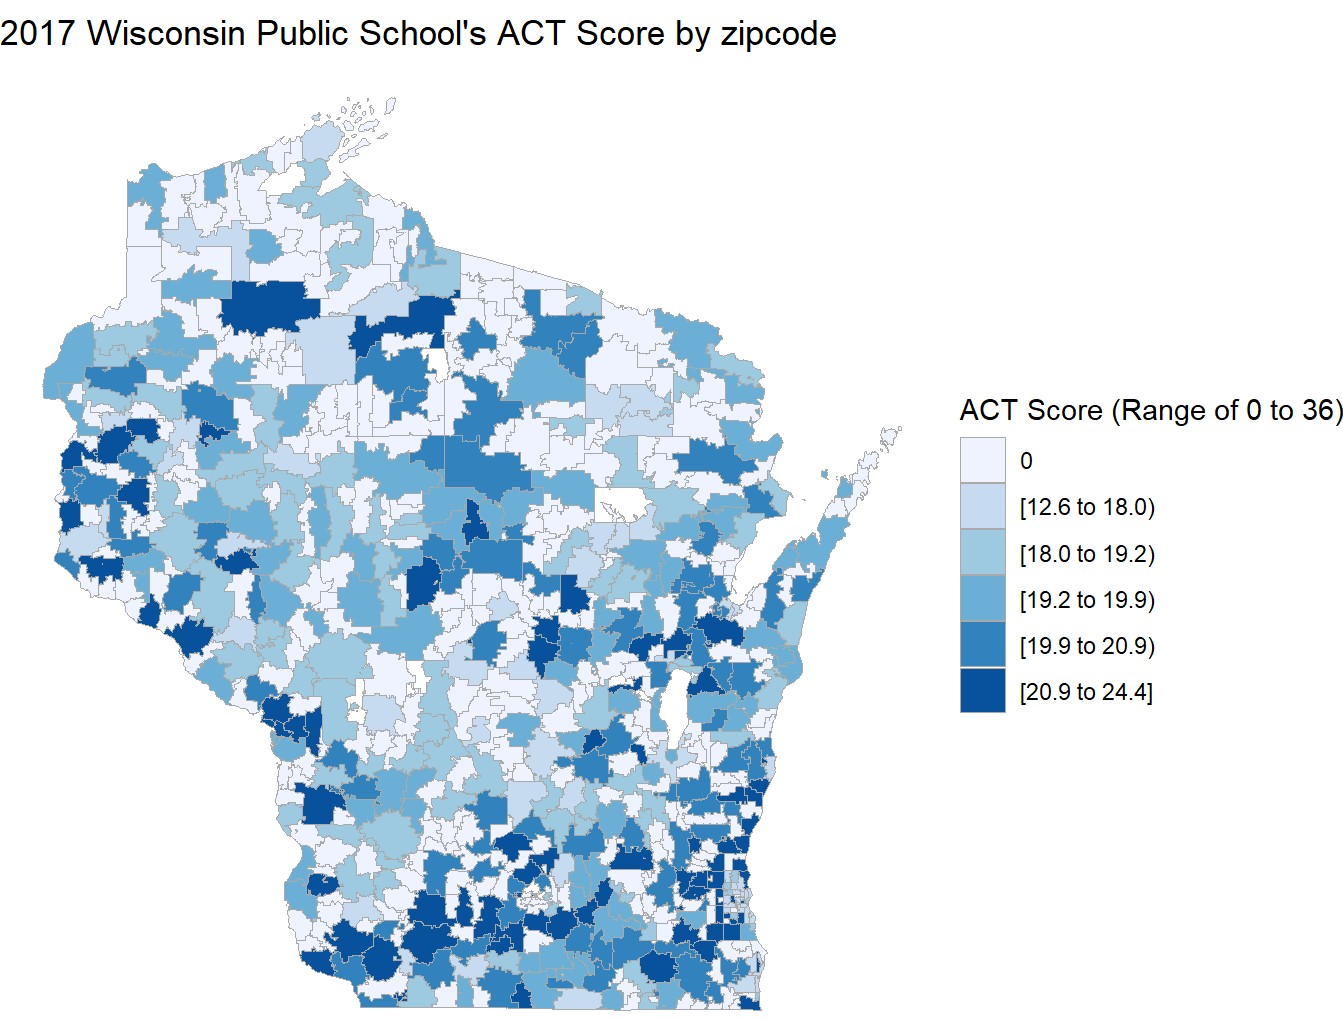
\includegraphics[width=1.0\linewidth]{2017_ACT_Score.jpg}
\end{center}
\caption{Plot for 2017 ACT Average score for Wisconsin's Public Schools}
\label{fig:long}
\label{fig:onecol}
\end{figure}

Comparing this data's figure (Figure 4) to Figure 3, similar patterns can already be observed between areas in Wisconsin with higher incomes and areas which have higher average ACT Scores.
This pattern is especially prevalent in inner city Milwaukee and its surrounding areas.
Comparing both graphs, it can be seen that inner city Milwaukee, an area of generally significantly low income, also has significant low ACT scores.
Contrasted with it's surrounding areas, of higher income, that have significantly high ACT scores. 

\section{STATISTICAL ANALYSIS}

To conduct our analysis, we decided to use two different multiple linear regression models for our two different output variables, ACT score and graduation rate. 

\subsection{Statistical Model for ACT Score}

\begin{figure}[h]
\begin{center}
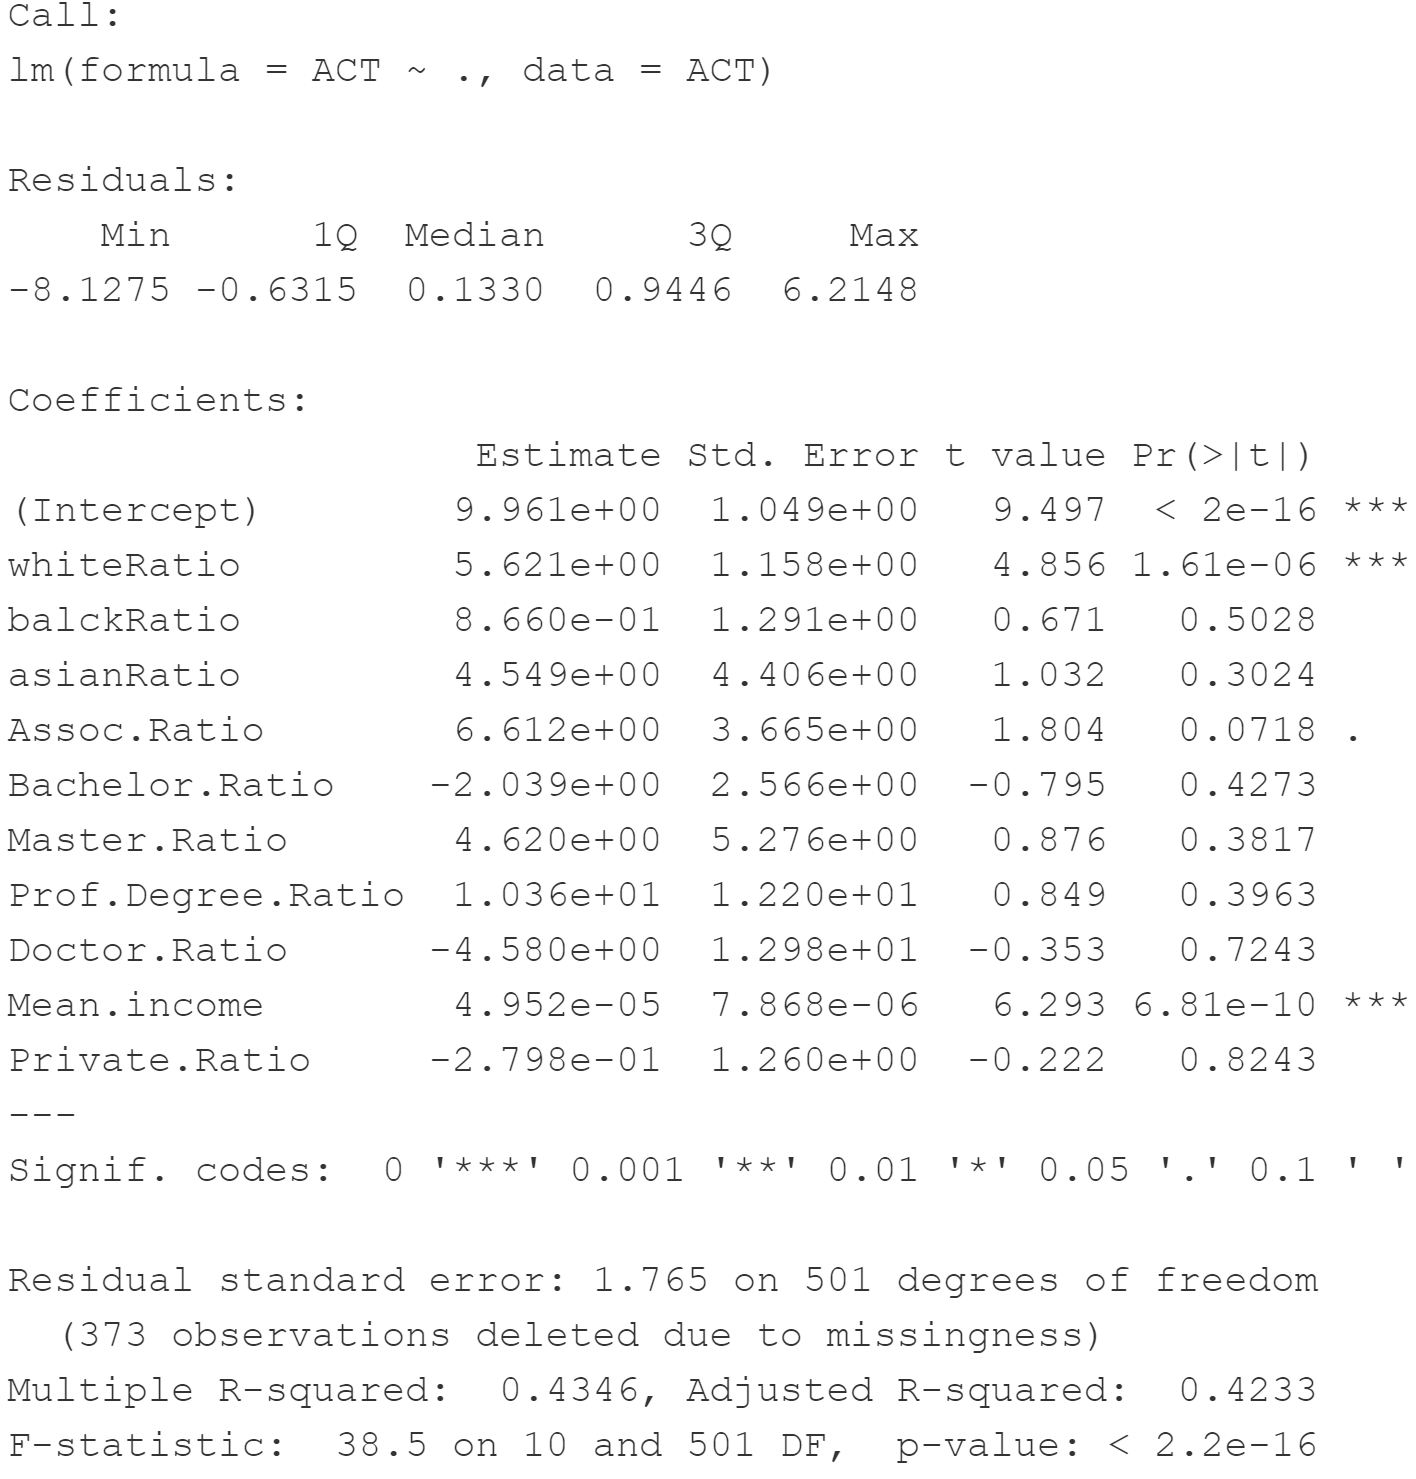
\includegraphics[width=1.0\linewidth]{Summary_ACT_All.PNG}
\end{center}
\caption{Linear Regression Model for ACT
  \newline Diagnostic Plots are located at the end of article}
\label{fig:long}
\label{fig:onecol}
\end{figure}

When making a linear model to analyze the relationship between our features and ACT score (See Fig. 5), we used a linear regression with ACT score as our dependent variable and demographic (White, Asian, Black ratio), parent's education level (Associate, Bachelor, Master, Prof.Degree, Doctor ratio of the zip code), mean income, and private school enrollment ratio as our independent variables.

The result shows that for the ACT test score, the significant variables were white ratio (p = 1.61e-16) along with mean income of the zip code (p = 6.81e-10).

We expected that mean income would have a significant effect on student's ACT Score, because wealthier students can afford to take the test several times, which has been known to increase a students' score. Besides that, wealthier students typically attend better-funded schools with a significant number of AP classes and are more likely to have access to tutors and standardized test preparation classes. 

Interestingly, the willingness of putting additional money on the children's education, proxied by private school enrollment rate, does not play a significant role.
Knowing that we only have the ACT score data for public schools and the willingness of investment toward education cannot only be illustrated by this simple factor, this result is not that surprising.

Note that, parent's education level is not significant in relation to student's ACT score, which is out of our expectation because we expected the higher the academic degree earned by parents, the higher the students' test scores. 

Interestingly, the white ratio is the only significant variable among the demographic, we believe this is because areas of higher income and thus better schools, tend to be areas with a higher white ratio, such as the suburbs. Additionally, Milwaukee has one of the highest rates of segregation in the United States, which leads to low-income areas full of minority populations that have poor quality schools, and thus poor educational outputs.
This factor could be influencing the model due to the large amount of Milwaukee Public Schools (MPS) that are represented in the data. When looking at the individual data points for MPS schools, many of their average ACT scores are significantly below the average. There are also significantly more schools in Milwaukee than any other area in Wisconsin. 

\begin{figure}[h]
\begin{center}
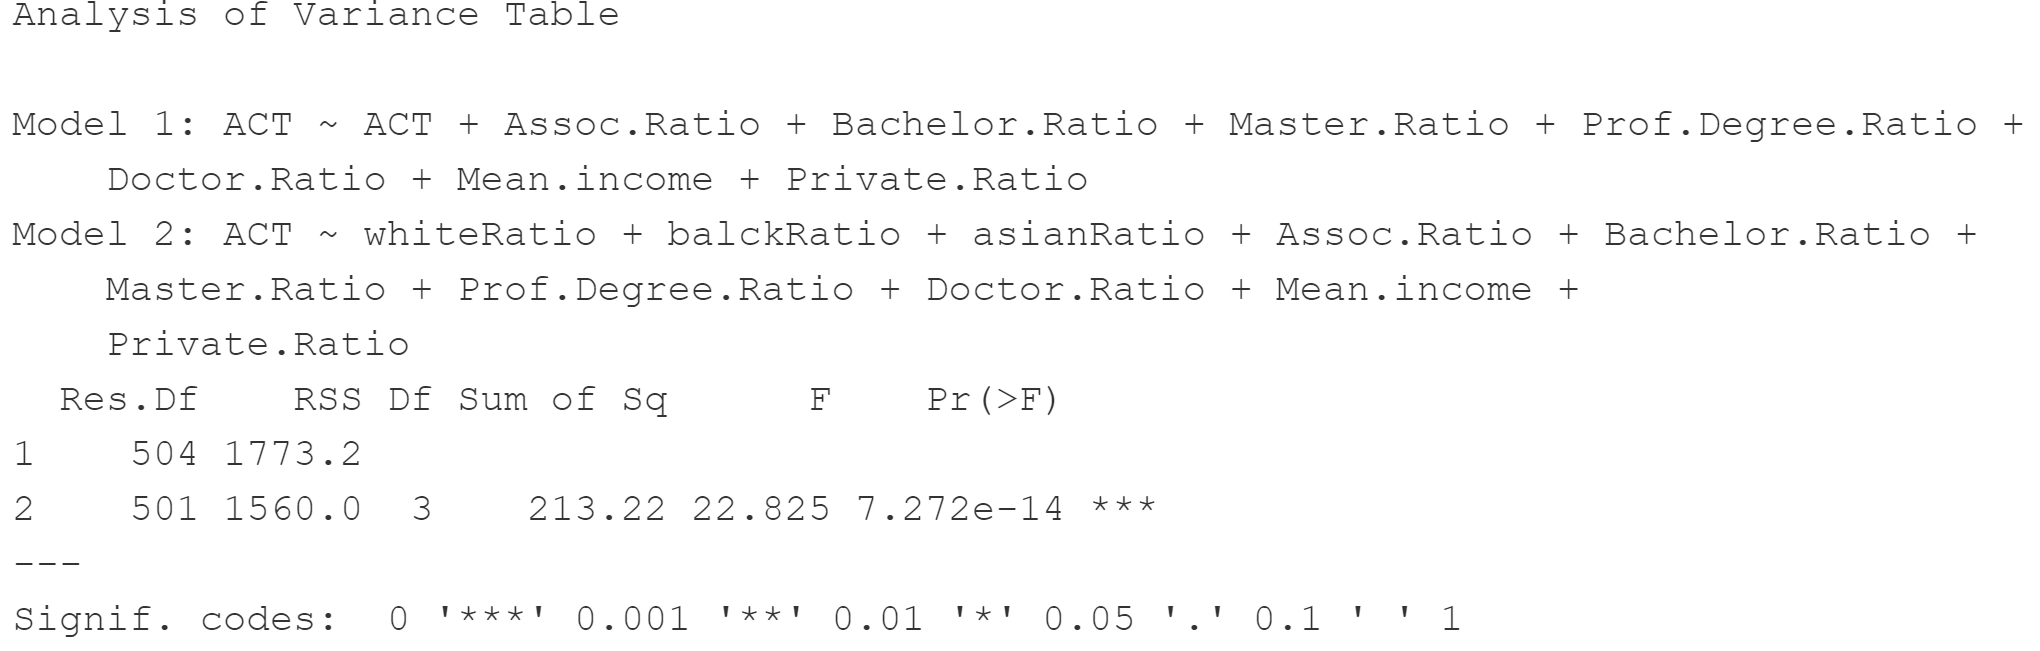
\includegraphics[width=1.0\linewidth]{ANOVA_ACT.PNG}
\end{center}
\caption{ANOVA table for checking significance of demographic feature.}
\label{fig:long}
\label{fig:onecol}
\end{figure}

For ANOVA analysis on the model with demographic feature and one without it (See Fig.6), we found that demographic information is significant (p = 7.272e-14) in relation to the linear model for students' ACT score, which shows that including demographic in our model influences students' ACT score.

To check how well our model represents the data, we plotted four diagnostic plots for our linear model for students' ACT score (See Fig.9).
Our first plot, Residuals vs Fitted, shows that our residuals have a linear relationship.
The residuals also appear to be mostly normally distributed as per the Q-Q plot with a few deviations present in the ends of the graph.

\subsection{Statistical Model for Graduation Rate}

\begin{figure}[h]
\begin{center}
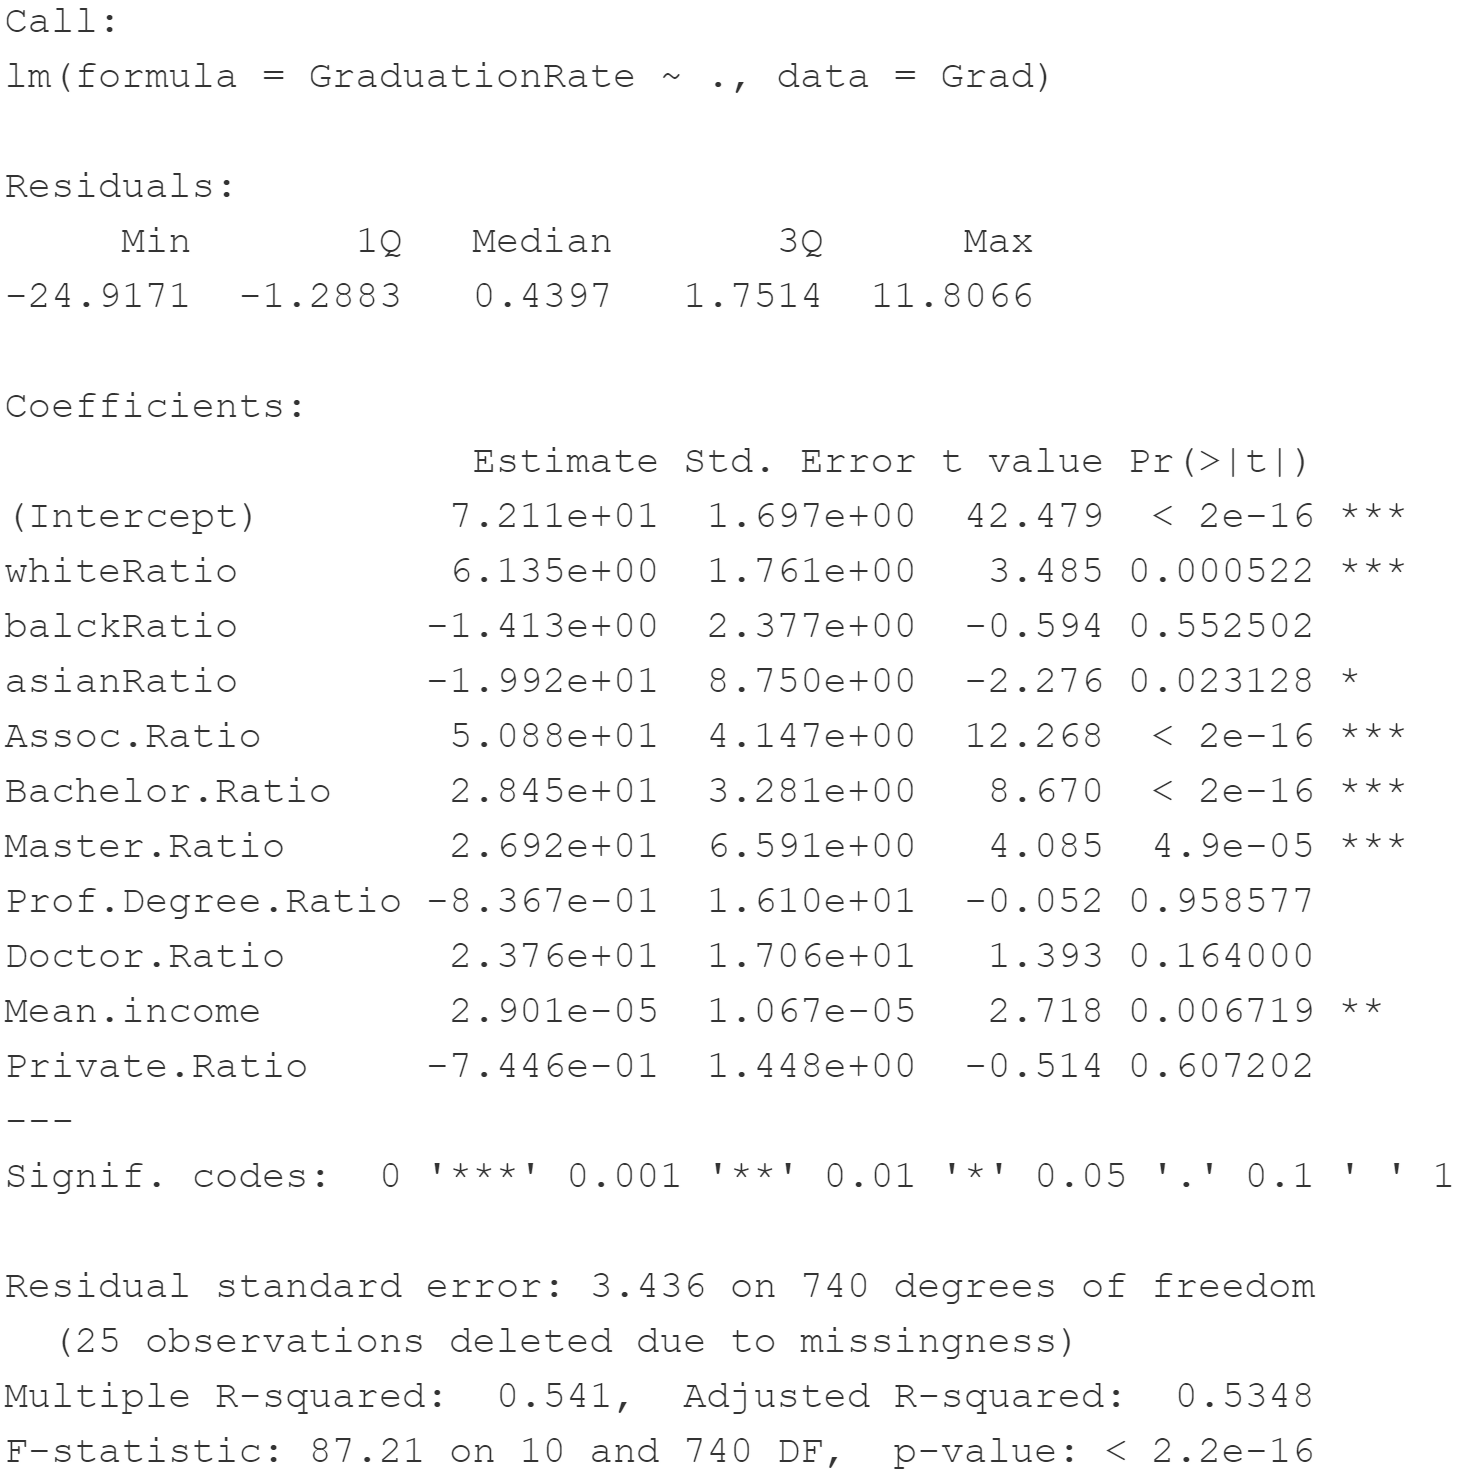
\includegraphics[width=1.0\linewidth]{Summary_Grad_All.PNG}
\end{center}
\caption{Linear Regression Model for Grad
  \newline Diagnostic Plots are located at the end of article}
\label{fig:long}
\label{fig:onecol}
\end{figure}

When making a linear model to analyze the relationship between our features and the output (See Fig. 7), it was found that the significant variables were the ratio of white people (p = 0.000522), the ratio of Asian people (p = 0.0231), the ratio of associate's (p $<$ 2e-16), bachelor's (p $<$ 2e-16), and masters (p = 4.9e-5) degrees, along with the mean income of the zip code (p = 0.00672). 

We expected that education levels of employees would be significant in relation to graduation rate, because we expected that parents (the employees) with higher levels of education would also want their children to pursue higher education and thus, have better educational outputs in high school. 
It is notable though that professional degrees and doctorates were not found to be significant, even though we still expected this trend to be relevant as education level of the parents increase. 

Interestingly, race also play a significant role in this model, especially the white ratio.
We suspect it is because better schools tend to be in areas with higher income and lower minority populations (suburbs), so schools with better educational outputs tend to have more white students.
As it was mentioned earlier, there is a significant problem with segregation in Milwaukee. Because of the segregation, there are zip codes in low-income areas that have significant minority populations. 
This factor could be influencing the model due to the large amount of Milwaukee zip codes that are present in the data compared to other areas which generally only have one or two zip codes represent the area. 

\begin{figure}[h]
\begin{center}
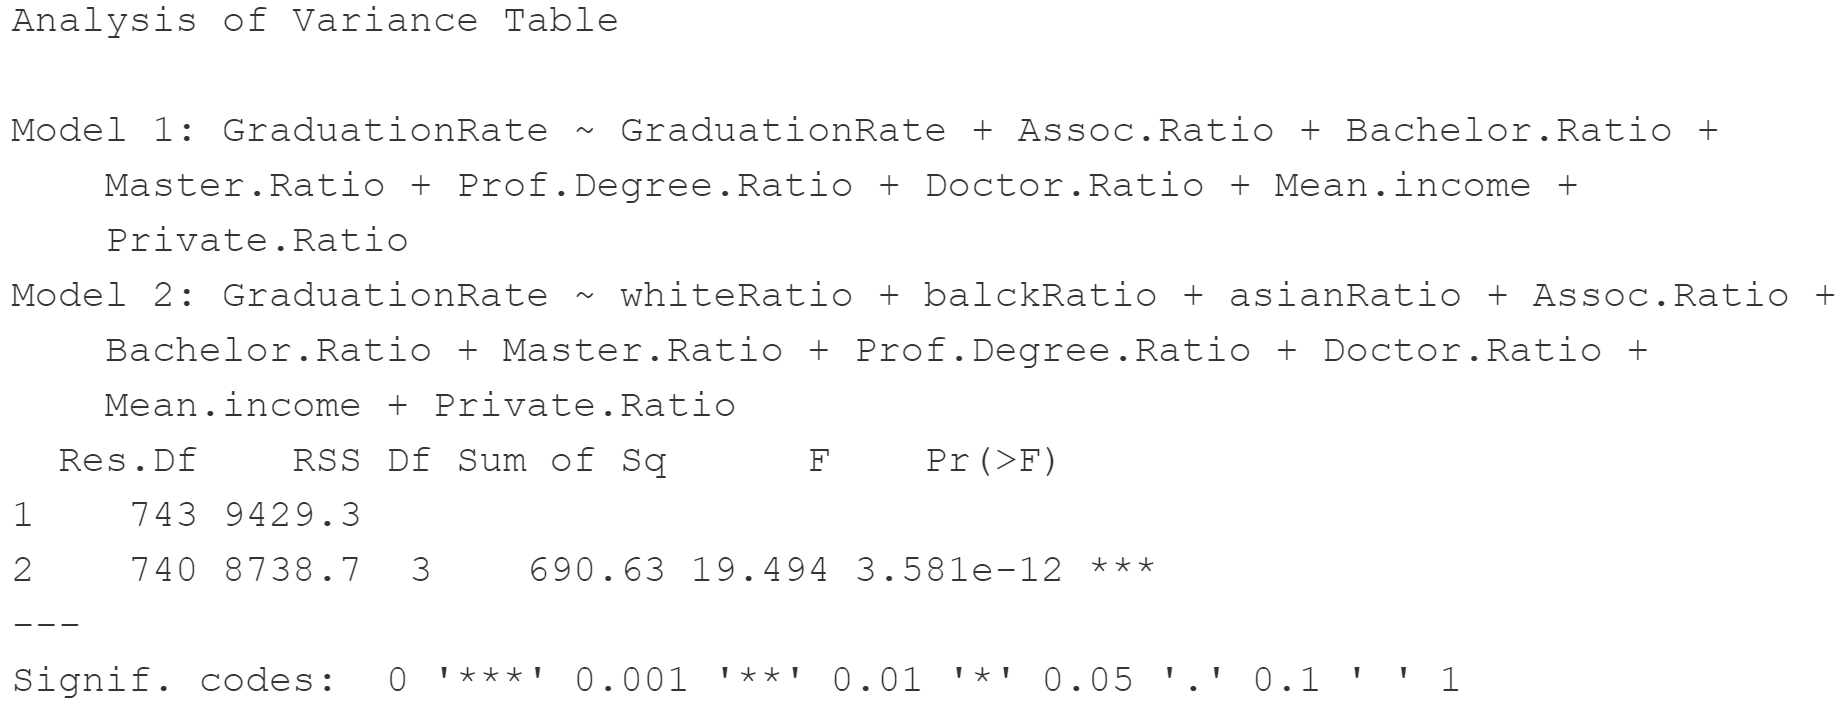
\includegraphics[width=1.0\linewidth]{ANOVA_Grad.PNG}
\end{center}
\caption{ANOVA table for checking significance of demographic feature}
\label{fig:long}
\label{fig:onecol}
\end{figure}

When conducting ANOVA test on the demographic information (See Fig. 8), we created two models, one that featured white ratio, Asian ratio, and black ratio and one that did not.
The ANOVA analysis was found to be significant (p=3.58e-12), which shows that the demographic information is significant in relation to the linear model for graduation rate.

The diagnostic plot for the data (See Fig. 10) appears relatively normal.
The residuals vs. fitted plot shows an indication of a linear relationship in the data, which is what we want.
The residuals also appear to be mostly normally distributed as per the Q-Q plot with a few deviations present in the ends of the graph. 

\section{LIMITATIONS}

The biggest limitation of our project is data limitation.
The best way to have conducted this research would have been to get data for each individual person and conduct analysis on the individual level.
Unfortunately, data such as this is just simply not available.
Because of this, we had to use zip codes, but for each of these it is only averages within a specific area.
Data such as this is not weighted to the area’s populations, so areas that are less populated are less resilient to outliers and therefore could have their averages easily affected by extreme high or low values. 

Furthermore, the ACT data we used was indexed by the zip code of the school.
This limited the data we were able to use, as we could only use zip codes that had a corresponding public school (and ACT score) in our analysis.
So, we were unable to use zip codes in which there was no school, even though there still may be students residing within that area.
Secondly, this data is not able to account for the zip codes in which students actually live, only where they go to school. 
There is often shifting of where students go to school, or students who live in a different zip code than the school they attend.
To deal with this issue, we tried to find zip codes of students attending each school, to better group the data, but we cannot group zip codes according to school districts because we were unable to find the data for this.
Moreover, we also tried to find the data set indicating mean income, parents' highest diploma, and demographic for each school, but the public schools do not need to report this data.
Researching more about this, the survey about income status of each student is restricted by Protection of Pupil Rights Amendment (PPRA), and so schools are unable to report this data (What is the..., n.d., [6]).

Additionally, it is almost impossible to find data for how much a parent invests in their child’s education such as prep class for ACT and hiring private tutors.
We could only use proxies such as mean income and private school enrollment, but that does not necessarily correlate to how much parents invest in a child's education.
Furthermore, the mean income include childless family incomes and we are not able to remove that from our data.


\section{CONCLUSIONS}

Overall, the two statistical model that we fitted state that the mean income of each household significantly affects a child's academic output.
Although, due to the existing limitation, we were not able to conclude the willingness to invest additional dollars towards children's education makes a significant difference on their academic success, we were able to show that the income, the implied wealth of parents, makes difference on the educational output of their children.

With the discovered relationship between parental wealth and the educational output, we are able to conclude that education might be able to be utilized as a tool to transfer the wealth of the parents’ generation to their kids, contributing toward the polarization.
Sadly, the education causes the silver spoon effect, and this is the time for the government to think about providing fair opportunities on education in order to combat the long-lasting societal problem, polarization.


\addtolength{\textheight}{-12cm}   % This command serves to balance the column lengths
                                  % on the last page of the document manually. It shortens
                                  % the textheight of the last page by a suitable amount.
                                  % This command does not take effect until the next page
                                  % so it should come on the page before the last. Make
                                  % sure that you do not shorten the textheight too much.

%%%%%%%%%%%%%%%%%%%%%%%%%%%%%%%%%%%%%%%%%%%%%%%%%%%%%%%%%%%%%%%%%%%%%%%%%%%%%%%%

%%%%%%%%%%%%%%%%%%%%%%%%%%%%%%%%%%%%%%%%%%%%%%%%%%%%%%%%%%%%%%%%%%%%%%%%%%%%%%%%



%%%%%%%%%%%%%%%%%%%%%%%%%%%%%%%%%%%%%%%%%%%%%%%%%%%%%%%%%%%%%%%%%%%%%%%%%%%%%%%%



\begin{thebibliography}{99}

\bibitem{c1} Rugaber, C. S. (2017, January 12). Pay gap between college grads and everyone else at a record. Retrieved November 27, 2019, from https://www.usatoday.com/story/money/2017/01/12/pay-gap-between-college-grads-and-everyone-else-record/96493348/.

\bibitem{c2} QCEW News Releases. (n.d.). Retrieved December 2, 2019, from https://www.bls.gov/cew/.

\bibitem{c3} Data Slices by Industry. (2016, June 21). Retrieved December 2, 2019, from \newline
https://data.bls.gov/cew/doc/access/csv\_data\_slices.htm\#ANNUAL\_LAYOUT.

\bibitem{c4} American FactFinder - Search. (2010, October 5). Retrieved December 2, 2019, from \newline https://factfinder.census.gov/faces/nav/jsf/pages/searchresults.xhtml?refresh=t.
"??::

\bibitem{c5} Wisconsin ACT scores 2017-18. (n.d.). Retrieved December 10, 2019, from https://wisinfo.com/milwaukee/database/2018/wisconsin-act-scores-2017-18/\#!/composite.desc.1/.

\bibitem{c6} What is the Protection of Pupil Rights Amendment (PPRA)? (n.d.). Retrieved December 10, 2019, from \newline https://studentprivacy.ed.gov/faq/what-protection-pupil-rights-amendment-ppra.

\end{thebibliography}

%%%%%%%%%%%%%%%%%%%%%%%%%%%%%%%%%%%%%%%%%%%%%%%%%%%%%%%%%%%%%%%%%%%%%%%%%%%%

\onecolumn

\begin{figure}[h]
\begin{center}
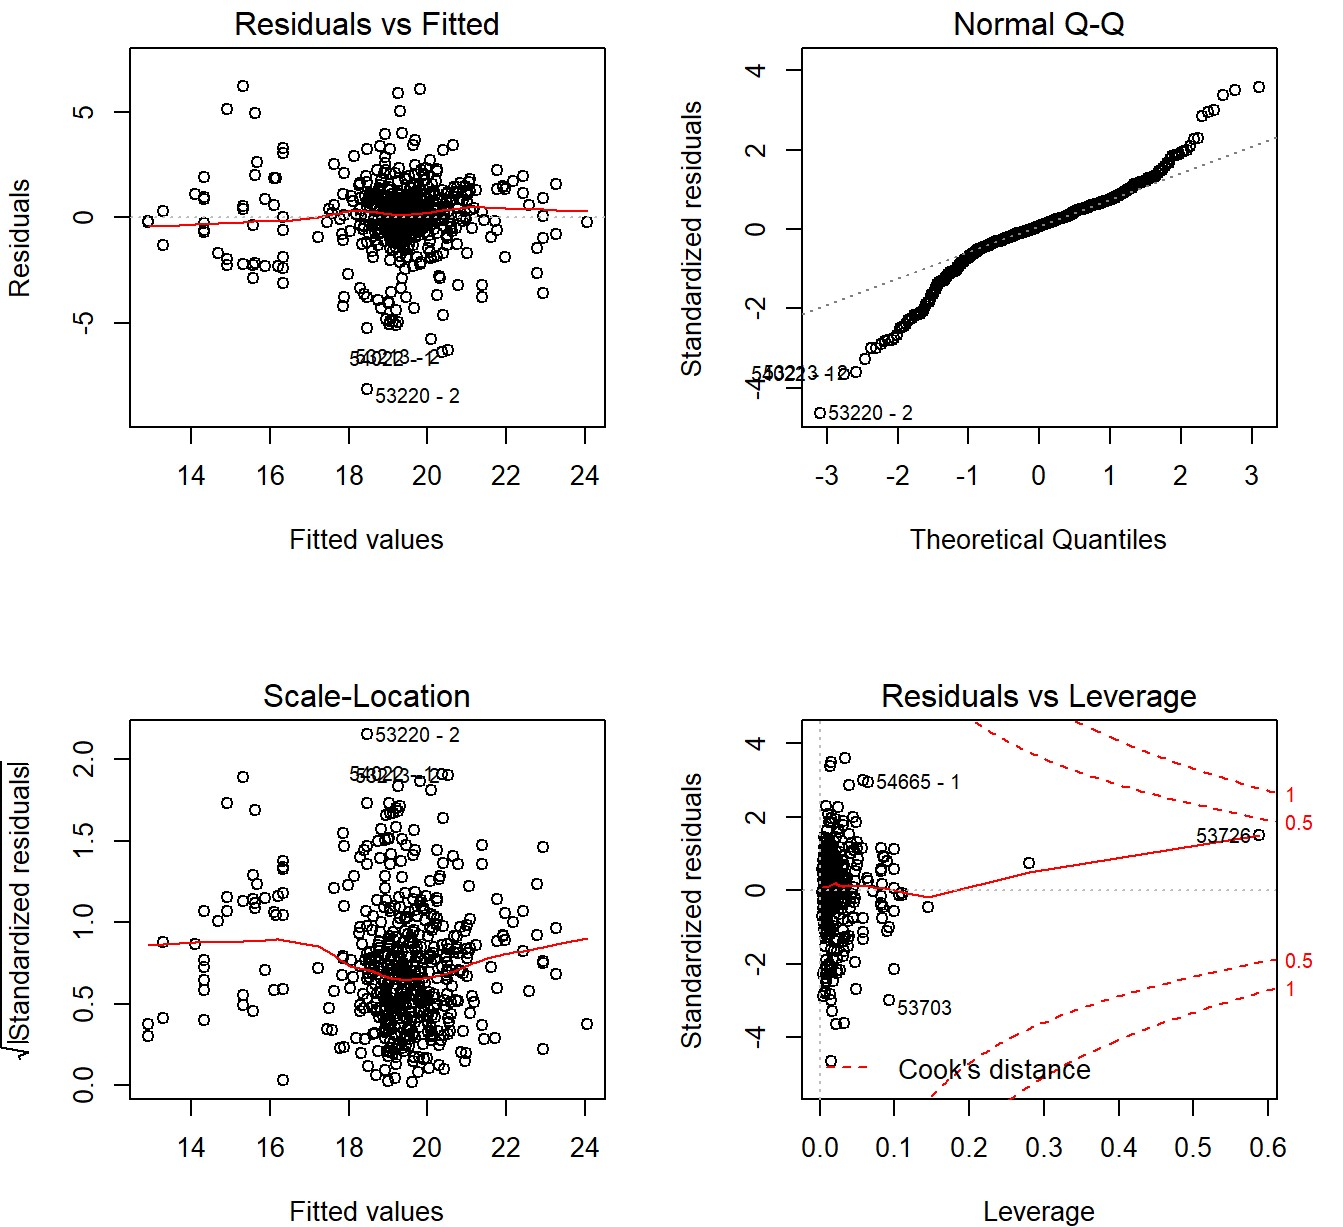
\includegraphics[width=\columnwidth]{DiagnosticPlot_ACT.jpg}
\end{center}
\caption{Diagnostic Plot for ACT Model}
\label{fig:short}
\end{figure}

\begin{figure}[h]
\begin{center}
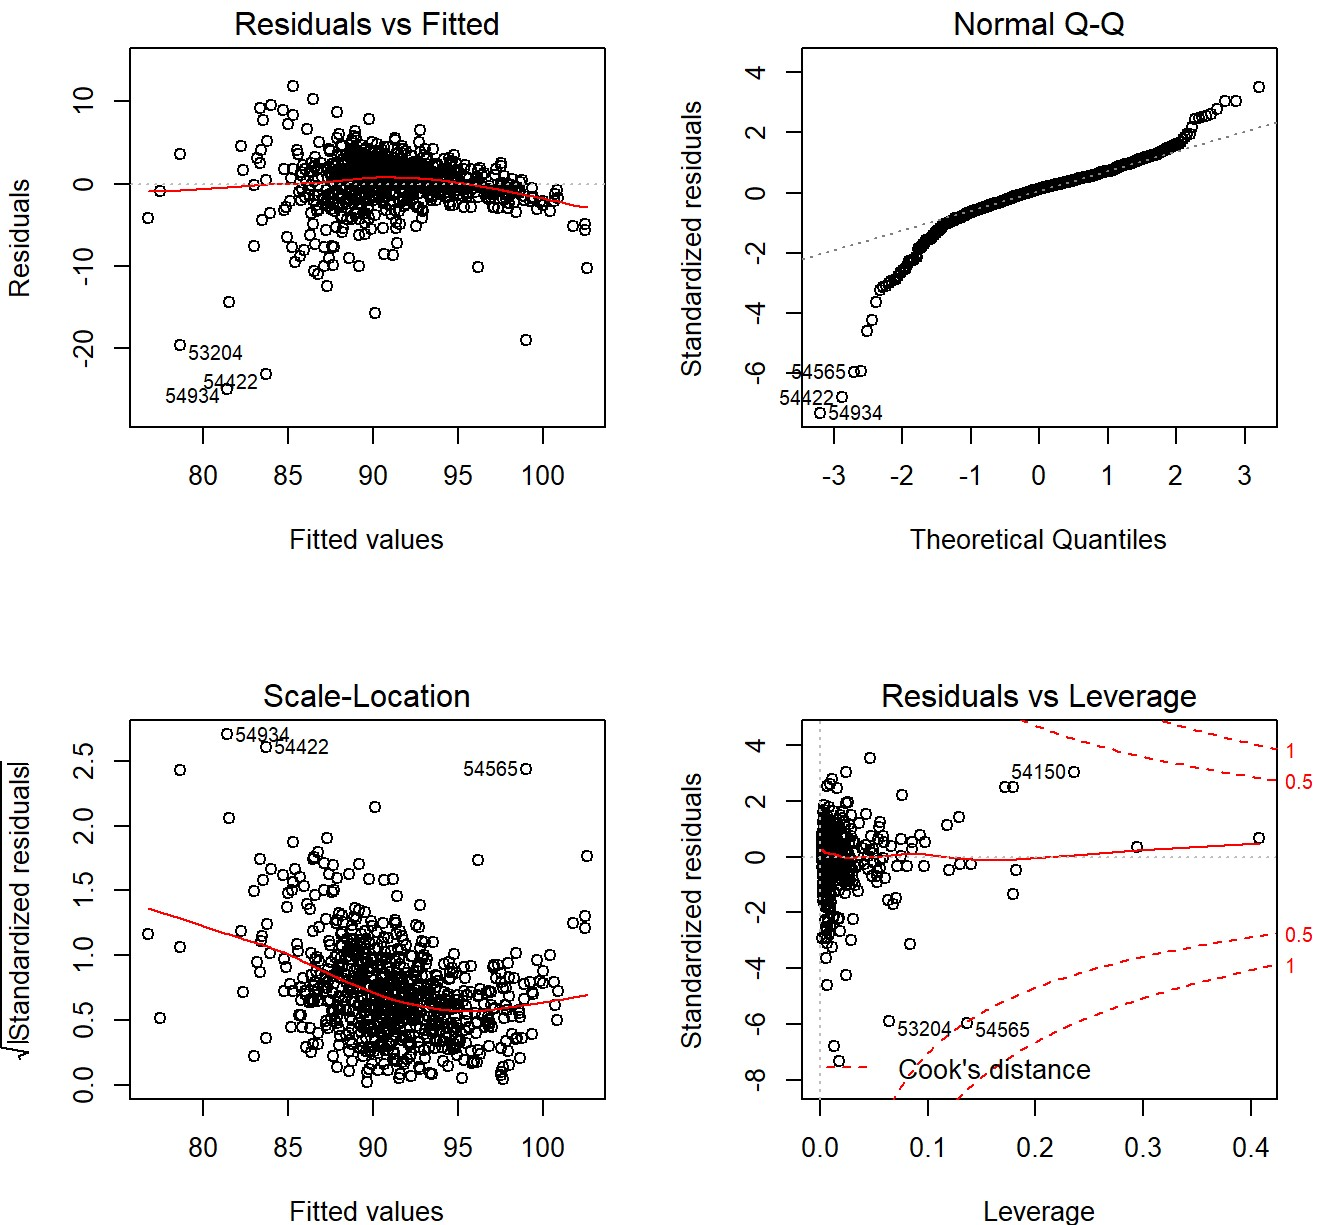
\includegraphics[width=\columnwidth]{DiagnosticPlot_Grad.jpg}
\end{center}
\caption{Diagnostic Plot for Graduation Rate Model}
\label{fig:short}
\end{figure}


\end{document}
